The implementation of the project was done in python. In general classes containing logic for different objects were implemented, for instance classes for polynomials, factorials, powers and so on were implemented. All classes were implemented from scratch and we want to stress that this makes some of the code redundant -- surely it is implemented by others before -- and inefficient -- no highly efficient methods are used, but only the most simple versions. The reason the classes were implemented from scratch anyways was to more deeply understand the problems arising within computer algebra, and during the process it became clear that even methods that are very simple in theory can cause several hours of implementation and many lines of code.

The implementation of Wilf-Zeilberger's method can be divided into mainly three parts: parsing, testing and methods. Parsing is when we read a string and convert this into classes or logic that is used in the rest of the code. This is mainly to ease testing of the methods that are implemented. Testing is when we test the methods and see that they behave as intended. Methods is the ''real'' code for the thesis, which is when we implement the logic that is described in chapter \ref{Ch: Theory}. In total the code produced in the thesis consists of about 2200 lines of code out of which about 50\% are the methods and classes used to implement the theory from chapter \ref{Ch: Theory}, 20\% is parsing and 30\% is testing. The testing is of course not necessary to keep for the sake of having functioning code, but is kept in order to show that the code has been tested.

The code consists of eight files that do different parts of the method. These are:

\begin{center}
  \begin{tabular}{C{1mm}C{3cm}|C{8cm}}
    &\textbf{File name}   & \textbf{What does the file include?} \\ \hline
    &Polynomial  & A class for polynomials with all methods that are needed. \\ \hline
    &Factor      & Classes for factorials and power (integer to the power of polynomials) \\ \hline
    &Expressions & Classes for storing expressions of factors, addends and fractional expressions \\ \hline
    &Main        & Main function that takes a parser and an input string as input and produces a \LaTeX file with a part proof where the user needs to do a few steps (which are indicated in the \LaTeX file) \\ \hline
    &Gosper      & Functions for running all steps of Gosper's algorithm and returning the solution \\ \hline
    &Get f       & Function for solving step 2 of Gosper's algorithm \\ \hline
    &Gaussian elimination & Function for solving a system of linear equations by using Gaussian elimination, which is used by Get f \\ \hline
    &Parsers     & Parser from a \LaTeX equation to the format that is used in the rest of the program \\
  \end{tabular}
\end{center}

The dependencies of the files can be drawn as follows where an arrow from $A$ to $B$ means that $B$ depends on $A$:
\begin{figure}[H]
\centering
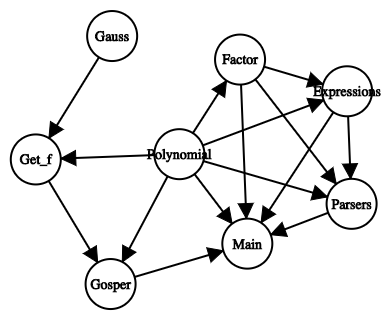
\includegraphics[width=0.6\textwidth]{images/dependency_graph.png}
\caption{Dependency graph of code}\label{Fig: DepGraph}
\end{figure}
Now that we have shown the general structure of the program, we will describe each of the important and interesting parts of the implementation. Firstly we will describe the structure used for parsing, thereafter we will discuss implementation of the methods needed for Wilf-Zeilberger's method. After that we will describe how a proof is written automatically and lastly we will shortly describe how testing has been done.

\section{Parsing}
In the project a several parsers are used. The parsers that have been implemented are shift-reduce parsers, which are a type of bottom-up parsers. In this type of parser a stack is used and a string is parsed character by character. When a character is read first the stack is reduced and then the character is pushed to the stack. That the stack is reduced means that if we read for instance a ''$+$'', then first all multiplications on the top of the stack are evaluated and first after that we push the ''$+$''. For more details and further explanation of a shift-reduce parser, see \reference{parser}.

In the code there are four parsers, which all read a string of a specific format and return either an object that the string represents or a string on another format. We are now going to describe the parsers with what they have as input and output, but first we need to describe an internal format that is used in the program to represent binomial coefficients, factorials and powers of integers. This format will in the rest of the report be referred to as \textit{the internal format} These three will be represented as follows:
\begin{center}
  \begin{tabular}{C{1mm}C{3cm}|C{4cm}|C{4cm}}
    &\textbf{What?}   & \textbf{Represented as:} & \textbf{Example:} \\ \hline
    &Factorial & $F[x]$, where $x$ is a polynomial & $(m+n)!$ is written as $F[n+m]$ \\ \hline
    &Binomial coefficient & $B[n,k]$ where $n,k$ are polynomials & $\binom{n+1}{k-1}$ is written as $B[n+1,k-1]$ \\ \hline
    &Power of integer & $P[a,n]$ where $a$ is an integer and $n$ is a polynomial & $2^n$ is written as $P[2,n]$ \\
  \end{tabular}
\end{center}

The parsers are described by the following table:
\begin{center}
  \begin{tabular}{C{1mm}C{3cm}|C{4cm}|C{4cm}}
    &\textbf{Parser}   & \textbf{Input format} & \textbf{Output format} \\ \hline
    &Polynomial parser & String with a polynomial, for instance ''n\^{}2+3km'' & Polynomial that the input string represents \\ \hline
    &Expression parser & String with an expression on the internal format, for instance ''(n!+k*m)/(n\^{}2+B[n,k])'' & Expression that the input string represents \\ \hline
    &\LaTeX parser     & String in \LaTeX format of an identity, for instance ''\textbackslash sum\_\{k=0\}\^{}n \textbackslash binom\{n\}\{k\}=2\^{}n'' & $F, a_k$ and the numerator and denominator of $\frac{a_k}{a_{k-1}}$ as the first step in the method \\ \hline
    &Internal format to \LaTeX parser  & String on the internal format & String on \LaTeX format \\
  \end{tabular}
\end{center}
\section{Gosper's algorithm}
\subsection{Finding p,q,r}
\subsection{Finding f}
\section{Proof generation}
